
\begin{figure}
    \centering
    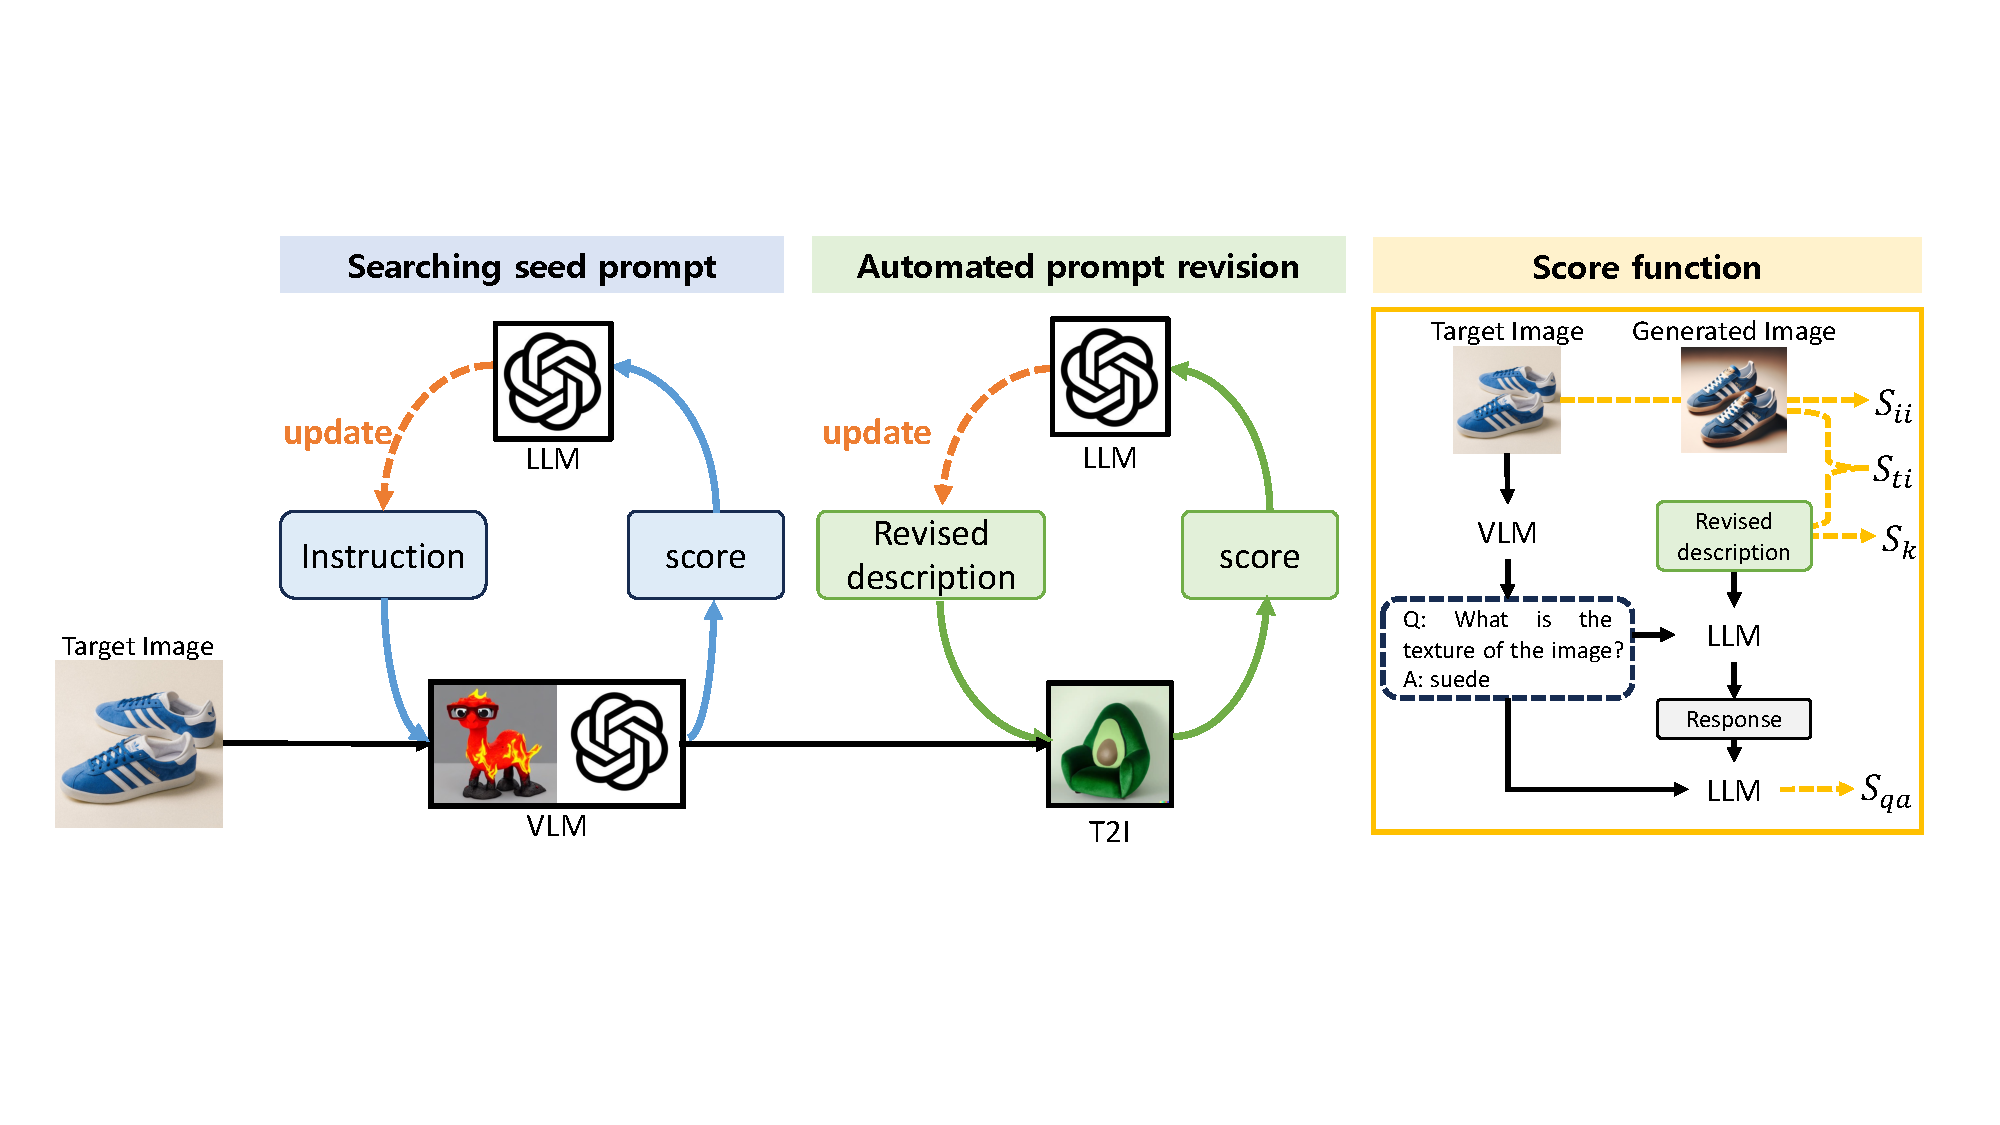
\includegraphics[width=0.99\textwidth]{figure_folder/concept.pdf}
    \vspace{-0.1in}
    \caption{\small \textbf{Concept figure of Automated Prompt Generation Pipeline (APGP).} The initial step is to optimize the instruction for the vision-large language model (VLM) in order to search for a high-quality seed prompt that is well-aligned to the target image in the CLIP space. Then, the prompt for text-to-image (T2I) system is optimized based on the score function to generate a high-risk prompt that describes the target image precisely. The optimizing score at the revision optimization step comprises four scores, image-image consistency $S_{ii}$, image-text alignment score $S_{ti}$, keyword penalty $S_k$, and self-generated QA score $S_{qa}$.}
    \label{fig:pipeline}
    \vspace{-0.23in}
\end{figure}